% 固定来源PDF印刷页50第12题的四个函数图象选项矢量重绘。
% 圆弧形状按题面函数及轴对称关系绘制；面板和坐标尺度仅作示意。
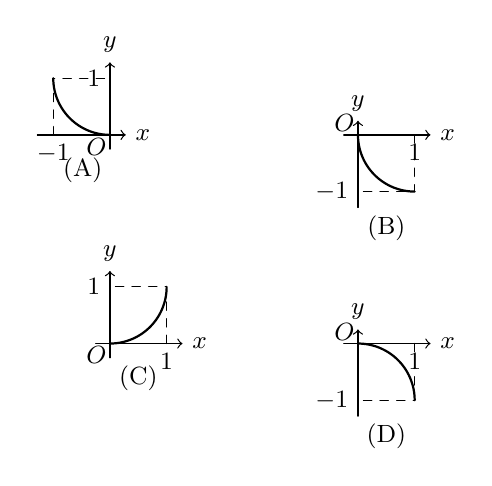
\begin{tikzpicture}[line width=.45pt,x=.72cm,y=.72cm,font=\small,line cap=round,line join=round]
  % (A) 给定函数 y=1-sqrt(1-x^2)，-1<=x<=0。
  \begin{scope}
    \draw[->] (-1.28,0)--(.28,0) node[right] {$x$};
    \draw[->] (0,-.25)--(0,1.28) node[above] {$y$};
    \draw[dashed] (-1,0)--(-1,1)--(0,1);
    \draw[thick,domain=0:90,samples=61,smooth,variable=\t]
      plot ({-sin(\t)},{1-cos(\t)});
    \node[below] at (-1,0) {$-1$};
    \node[left] at (0,1) {$1$};
    \node[below left,inner sep=1pt] at (0,0) {$O$};
    \node at (-.48,-.62) {(A)};
  \end{scope}

  % (B) 对(A)关于 y=x 对称的反函数图象。
  \begin{scope}[xshift=3.15cm]
    \draw[->] (-.25,0)--(1.28,0) node[right] {$x$};
    \draw[->] (0,-1.28)--(0,.25) node[above] {$y$};
    \draw[dashed] (1,0)--(1,-1)--(0,-1);
    \draw[thick,domain=0:90,samples=61,smooth,variable=\t]
      plot ({1-cos(\t)},{-sin(\t)});
    \node[below] at (1,0) {$1$};
    \node[left] at (0,-1) {$-1$};
    \node[above left,inner sep=1pt] at (0,0) {$O$};
    \node at (.5,-1.64) {(B)};
  \end{scope}

  % (C) 正值象限的相邻弧形选项。
  \begin{scope}[yshift=-2.65cm]
    \draw[->] (-.25,0)--(1.28,0) node[right] {$x$};
    \draw[->] (0,-.25)--(0,1.28) node[above] {$y$};
    \draw[dashed] (1,0)--(1,1)--(0,1);
    \draw[thick,domain=0:90,samples=61,smooth,variable=\t]
      plot ({sin(\t)},{1-cos(\t)});
    \node[below] at (1,0) {$1$};
    \node[left] at (0,1) {$1$};
    \node[below left,inner sep=1pt] at (0,0) {$O$};
    \node at (.5,-.62) {(C)};
  \end{scope}

  % (D) 第四象限的另一种端点切向示意。
  \begin{scope}[xshift=3.15cm,yshift=-2.65cm]
    \draw[->] (-.25,0)--(1.28,0) node[right] {$x$};
    \draw[->] (0,-1.28)--(0,.25) node[above] {$y$};
    \draw[dashed] (1,0)--(1,-1)--(0,-1);
    \draw[thick,domain=0:90,samples=61,smooth,variable=\t]
      plot ({sin(\t)},{cos(\t)-1});
    \node[below] at (1,0) {$1$};
    \node[left] at (0,-1) {$-1$};
    \node[above left,inner sep=1pt] at (0,0) {$O$};
    \node at (.5,-1.64) {(D)};
  \end{scope}
\end{tikzpicture}
